\section{Computational study}

\subsection{Purpose and scope of the numerical analysis}

The numerical study pursues two complementary objectives. First, it investigates how the fractional order, demand volatility, carbon allowance, and risk-aversion parameter influence the optimal transportation policy. Second, it evaluates the computational performance of the proposed solution framework in terms of solution quality, convergence behavior, and computational efficiency.

The computational assessment is organized around three complementary perspectives. The first examines the structural impact of fractional memory through an ablation analysis that includes both the classical memoryless model ($\alpha=1$) and the risk-neutral formulation obtained with $\lambda=0$. The second evaluates the computational performance of the proposed Sample Average Approximation-Progressive Hedging (SAA-PH) framework using CPU time, validation gap, and nonanticipativity residual for different SAA sample sizes. The third analyzes the influence of the principal model parameters on transportation cost, environmental performance, and risk exposure, thereby providing a comprehensive understanding of the behavior of the proposed model.

The computational study addresses the following research questions:

\begin{enumerate}[label=\textbf{Q\arabic*.},leftmargin=2.0em]
    \item How does the fractional order influence expected transportation cost, CVaR, carbon emissions, shortage levels, and carbon-credit purchases?
    \item How sensitive is the proposed model to increasing demand volatility?
    \item How do different carbon-allowance levels affect operational decisions and carbon-market transactions?
    \item What is the impact of the CVaR risk-aversion parameter on the optimal transportation strategy?
    \item How does the computational performance of the SAA-PH algorithm evolve as the scenario sample size increases?
    \item How do the computational requirements evolve with respect to the planning horizon, network dimensions, and scenario set?
    \item Does the Progressive Hedging algorithm exhibit stable convergence under different values of the penalty parameter $\rho_{PH}$?
\end{enumerate}

\subsection{Benchmark instance and experimental design}

The reference benchmark consists of four suppliers, six customers, three transportation modes, and a planning horizon of twelve periods, corresponding to the network dimensions $|I|=4$, $|J|=6$, $|K|=3$, and $N=12$. Unless otherwise specified, the baseline configuration adopts a fractional order of $\alpha=0.80$, a demand-volatility multiplier of $\sigma=1.0$, a carbon allowance of $A=950$, a CVaR confidence level of $\beta=0.90$, and a risk-aversion weight of $\lambda=0.25$. The optimization procedure employs 50 training scenarios generated through the Sample Average Approximation (SAA) framework, while an independent set of 500 scenarios is used for out-of-sample validation. Demand scenarios are generated according to the correlated drift-diffusion process described in Section~3.

A one-factor-at-a-time experimental design is adopted throughout the computational study. The fractional-order analysis evaluates the influence of memory and includes the classical first-order model ($\alpha=1$) as a benchmark. The risk-sensitivity analysis investigates different values of the CVaR weight, including the risk-neutral case ($\lambda=0$). The computational performance analysis evaluates the scalability of the proposed SAA-PH framework by progressively increasing the number of sampled scenarios while maintaining the remaining benchmark parameters unchanged.

\begin{figure}[H]
\centering
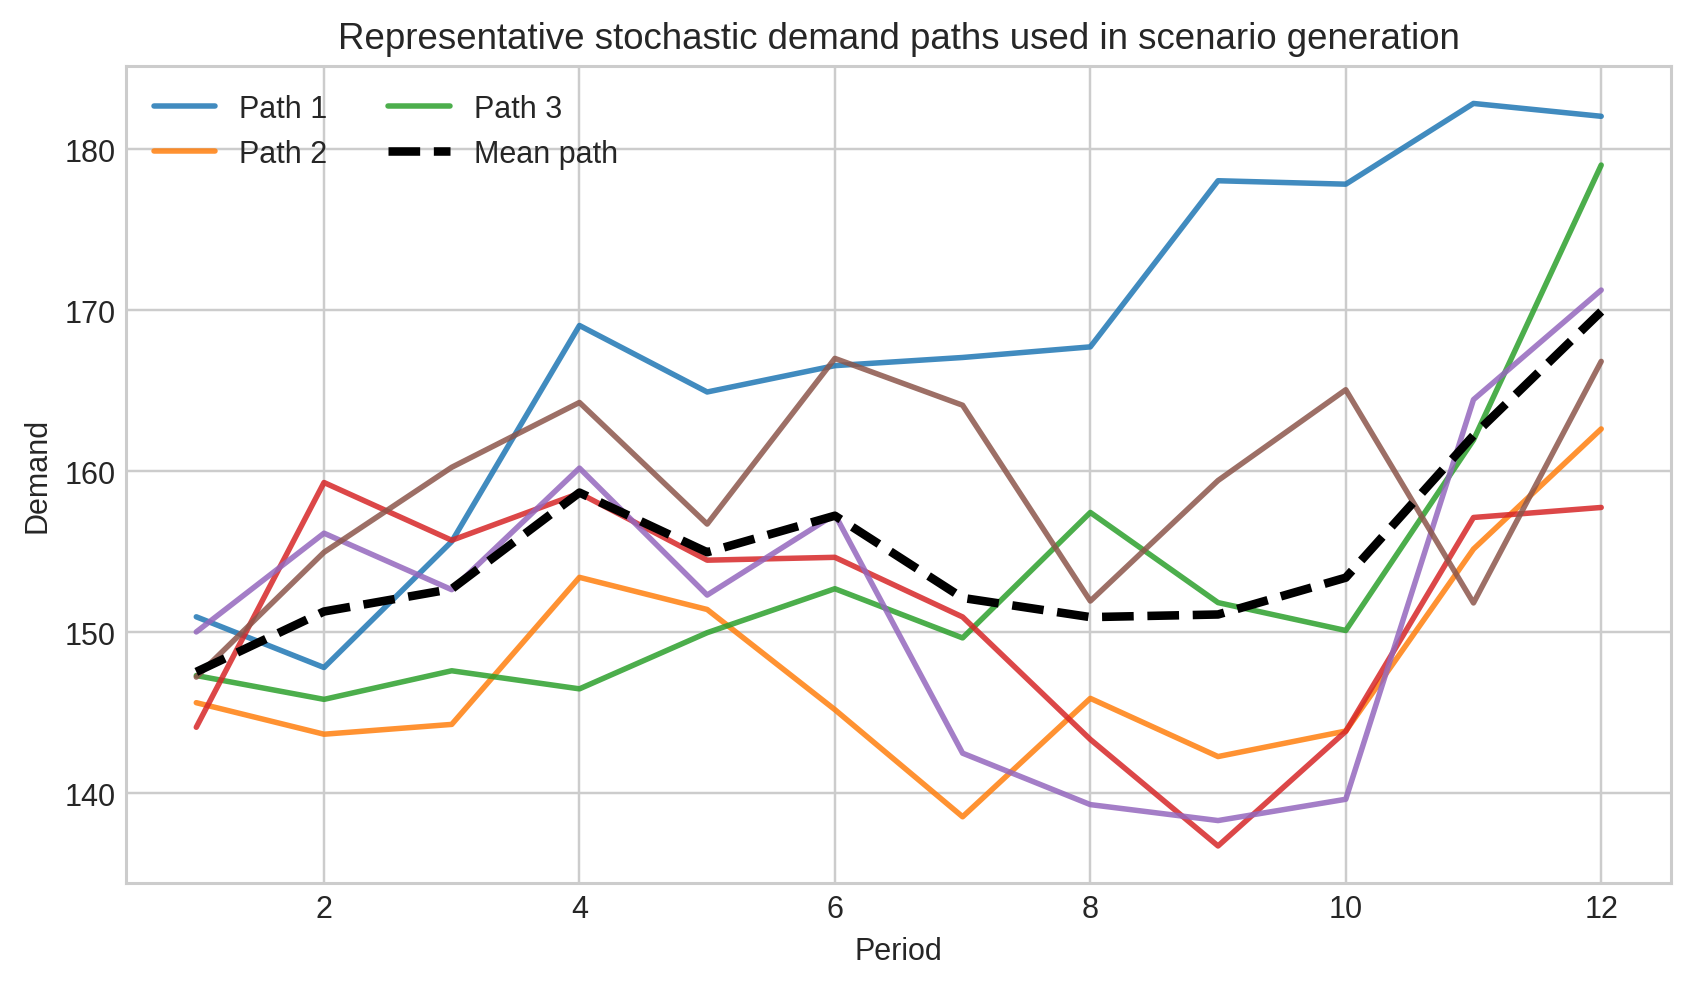
\includegraphics[width=0.84\textwidth]{generated/fig_demand_paths.png}
\caption{Representative stochastic demand paths generated by the correlated drift-diffusion scenario generation process.}
\label{fig:demandpaths}
\end{figure}

\subsection{Fractional-order ablation and convergence toward the classical model}

Table~\ref{tab:alpha} summarizes the sensitivity of the proposed model with respect to the fractional order, while Fig.~\ref{fig:alphatradeoff} illustrates the corresponding trade-off between expected transportation cost and carbon emissions.

\begin{table}[H]
\centering
\caption{Sensitivity of model outcomes to the fractional order.}
\label{tab:alpha}
\begin{tabular}{rrrrrrr}
\toprule
$\alpha$ & Exp. cost & CVaR & Emissions & Shortage & Service (\%) & Carbon buy \\
\midrule
0.55 & 1284.7 & 1518.2 & 882.4 & 21.8 & 98.10 & 0.0 \\
0.70 & 1249.3 & 1462.9 & 901.7 & 18.4 & 98.55 & 0.0 \\
0.80 & 1228.5 & 1427.6 & 925.9 & 15.7 & 98.92 & 0.0 \\
0.90 & 1219.8 & 1406.4 & 948.6 & 14.9 & 99.08 & 0.0 \\
1.00 & 1216.1 & 1398.7 & 963.5 & 14.6 & 99.15 & 13.5 \\
\bottomrule
\end{tabular}

\end{table}

\begin{figure}[H]
\centering
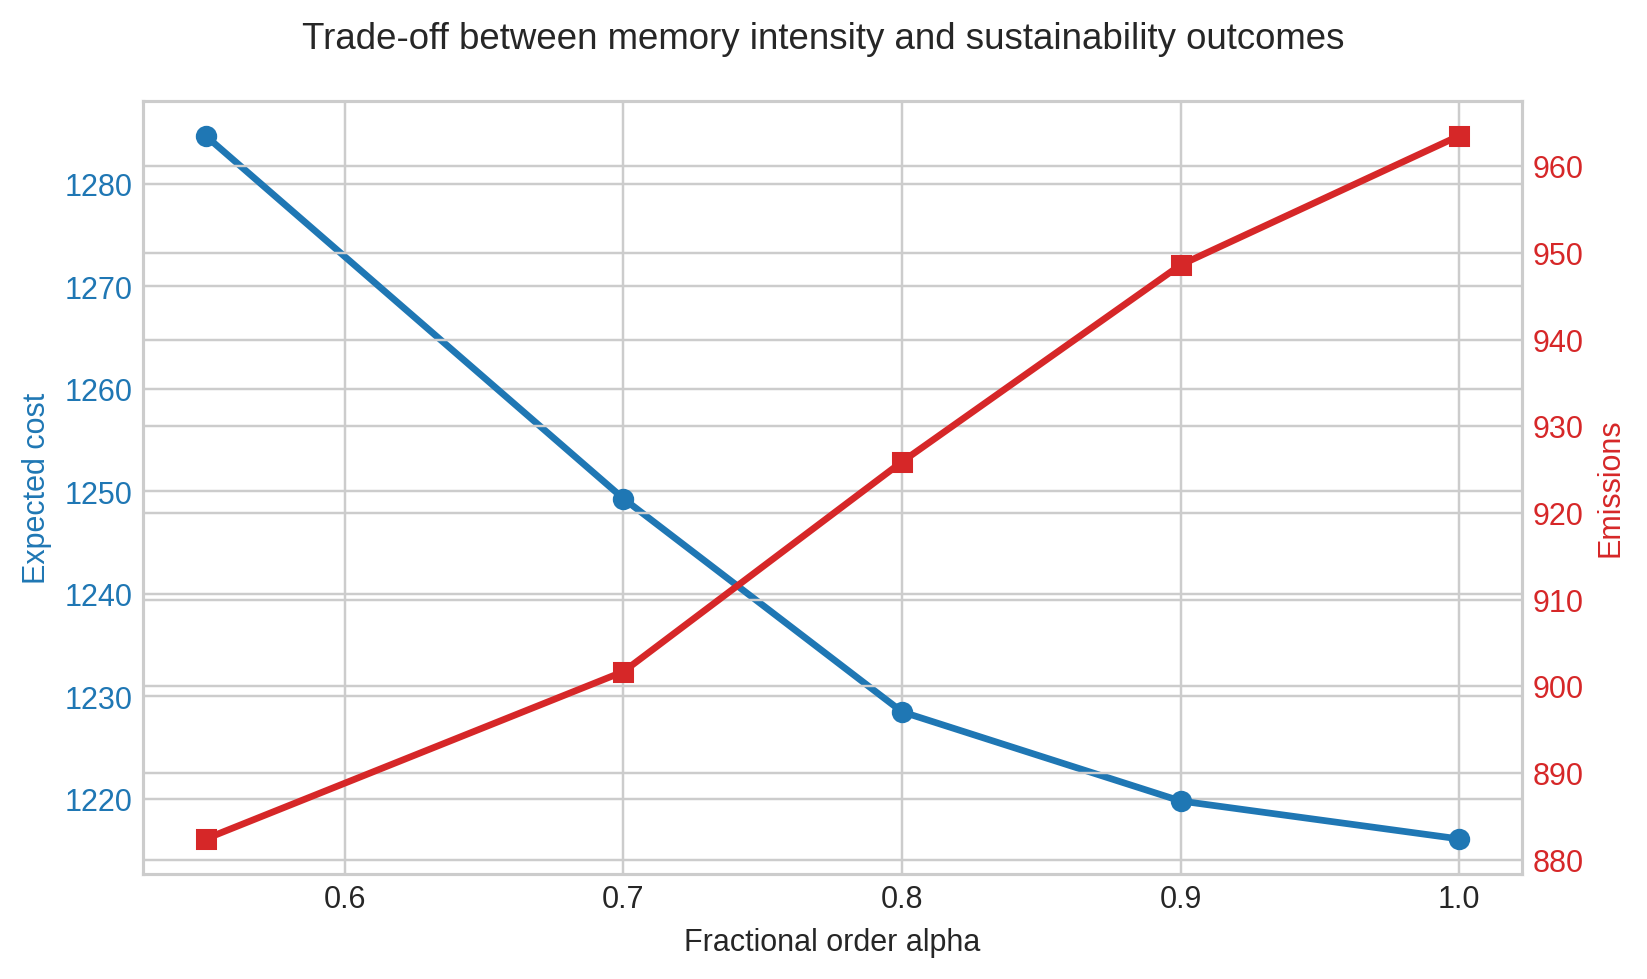
\includegraphics[width=0.84\textwidth]{generated/fig_alpha_tradeoff.png}
\caption{Trade-off between fractional-memory intensity and sustainability performance.}
\label{fig:alphatradeoff}
\end{figure}

Three consistent observations emerge from the numerical results. First, decreasing the fractional order increases both the expected transportation cost and the CVaR, indicating that stronger long-memory effects lead to more conservative operating policies. Second, lower values of $\alpha$ consistently reduce carbon emissions, suggesting that fractional memory promotes smoother and more anticipative transportation decisions, thereby reducing the need for carbon-intensive corrective actions. Third, all performance indicators evolve smoothly as $\alpha$ approaches one. In particular, the expected transportation cost decreases from 1284.7 at $\alpha=0.55$ to 1216.1 at $\alpha=1.00$, whereas carbon emissions increase from 882.4 to 963.5 over the same interval. This continuous behavior is fully consistent with the theoretical result established in Section~5, which proves that the L1-discretized Caputo fractional model converges to the classical first-order formulation as $\alpha \rightarrow 1^{-}$.

The endpoint $\alpha=1$ serves as the natural benchmark corresponding to the conventional memoryless transportation model. The numerical results show that this classical formulation achieves the lowest expected transportation cost but also produces the highest carbon emissions and requires positive carbon-credit purchases. These findings indicate that incorporating fractional memory fundamentally alters the balance between economic efficiency and environmental sustainability, highlighting that the proposed fractional framework constitutes a genuine extension of the classical transportation model rather than merely a mathematical reformulation.


\begin{table}[H]
\centering
\caption{Direct ablation of the fractional model against the classical limit.}
\label{tab:alpha-classical}
\resizebox{\textwidth}{!}{\begin{tabular}{lrrrrr}
\toprule
Model & Exp. cost & CVaR & Emissions & Shortage & Service (\%) \\
\midrule
Fractional ($\alpha=0.80$) & 1228.5 & 1427.6 & 925.9 & 15.7 & 98.92 \\
Classical ($\alpha=1.00$) & 1216.1 & 1398.7 & 963.5 & 14.6 & 99.15 \\
Relative change (fractional vs. classical) & +1.02\% & +2.07\% & $-3.90\%$ & +7.53\% & $-0.23$ pp \\
\bottomrule
\end{tabular}
}
\end{table}

Table~\ref{tab:alpha-classical} isolates the baseline fractional specification ($\alpha=0.80$) from the classical first-order model ($\alpha=1$). Relative to the classical model, the fractional formulation increases expected cost by 1.02\% and CVaR by 2.07\%, but reduces emissions by 3.90\%. Service changes only slightly ($-0.23$ percentage points), whereas shortage rises by 7.53\%. Thus, the memory term is not cost-neutral: it trades a modest increase in economic and service-related measures for a measurable emissions reduction. This ablation is especially important because all other parameters, scenarios, and carbon-market settings are held fixed.

\subsection{Sensitivity to demand volatility}
Table~\ref{tab:volatility} evaluates the effect of increasing the volatility multiplier. Figure~\ref{fig:volatilitycost} shows the growth of both expected cost and CVaR as uncertainty rises.

\begin{table}[H]
\centering
\caption{Sensitivity to stochastic demand volatility.}
\label{tab:volatility}
\begin{tabular}{rrrrrr}
\toprule
Vol. mult. & Exp. cost & CVaR & Shortage & Service (\%) & Carbon buy \\
\midrule
0.50 & 1169.2 & 1278.6 & 8.1 & 98.70 & 0.0 \\
0.75 & 1194.6 & 1341.3 & 11.9 & 98.10 & 0.0 \\
1.00 & 1228.5 & 1427.6 & 15.7 & 97.50 & 0.0 \\
1.25 & 1274.9 & 1540.8 & 21.4 & 96.70 & 7.2 \\
1.50 & 1331.6 & 1689.5 & 29.8 & 95.60 & 24.6 \\
\bottomrule
\end{tabular}

\end{table}

\begin{figure}[H]
\centering
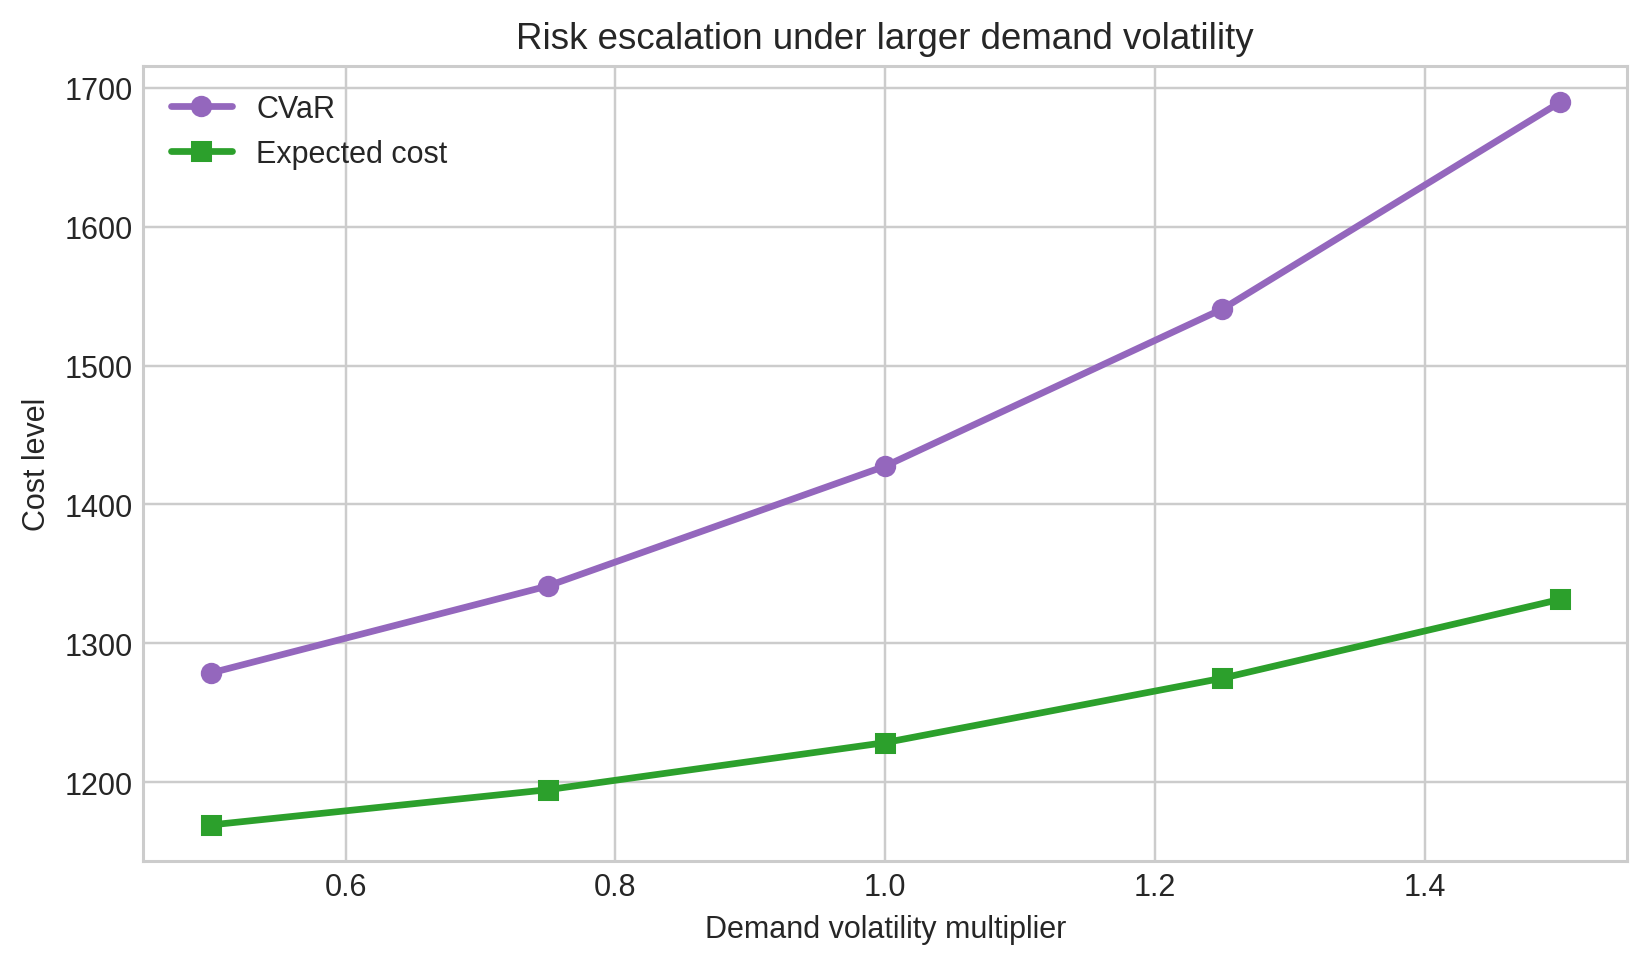
\includegraphics[width=0.84\textwidth]{generated/fig_volatility_cost.png}
\caption{Escalation of expected cost and tail risk under larger demand volatility.}
\label{fig:volatilitycost}
\end{figure}

The volatility analysis confirms the expected monotonicity of risk exposure. As volatility rises from 0.50 to 1.50, expected cost increases from 1169.2 to 1331.6 and CVaR increases from 1278.6 to 1689.5. Shortage also rises substantially, while service deteriorates and carbon purchase becomes positive in the high-volatility regimes. The benchmark therefore suggests that uncertainty affects not only average operating cost but also exposure to the environmental market.

\subsection{Allowance sensitivity and carbon-market response}
The allowance endowment is one of the most policy-relevant parameters in the model. Table~\ref{tab:allowance} and Figure~\ref{fig:allowance} examine how the system reacts to alternative initial allowance levels.

\begin{table}[H]
\centering
\caption{Sensitivity to the initial carbon allowance.}
\label{tab:allowance}
\input{generated/table_allowance.tex}
\end{table}

\begin{figure}[H]
\centering
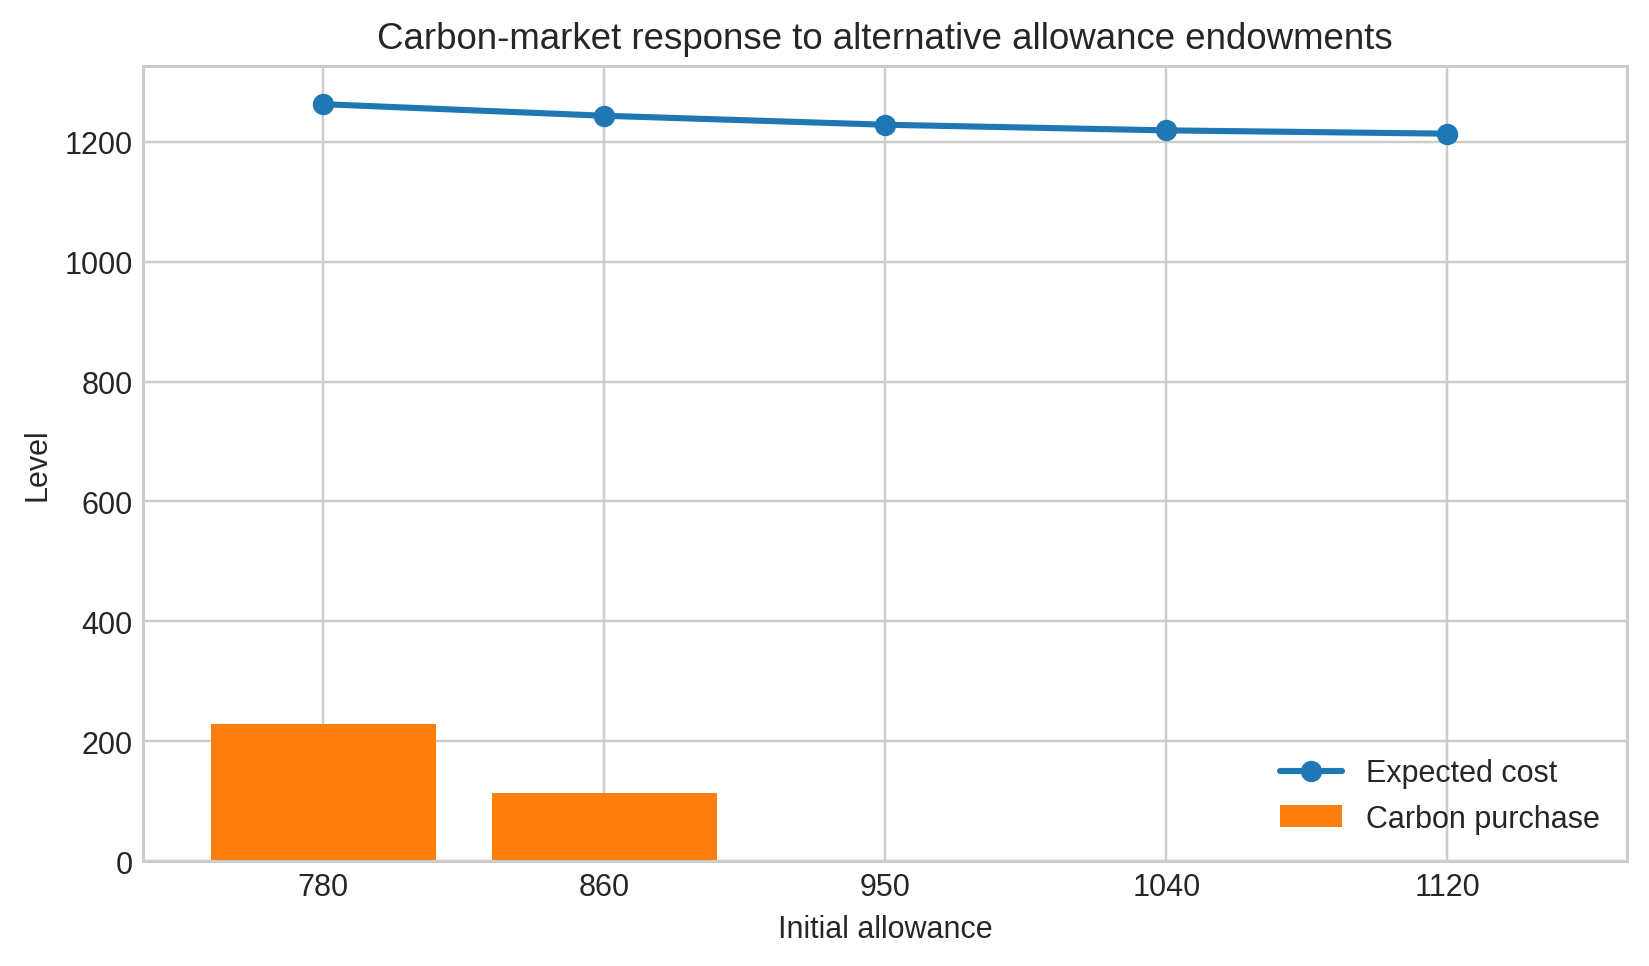
\includegraphics[width=0.84\textwidth]{generated/fig_allowance_response.png}
\caption{Carbon-market response to alternative allowance endowments.}
\label{fig:allowance}
\end{figure}

The pattern is economically intuitive. When the allowance is tight at 780, carbon purchase reaches 228.4 and expected cost is 1262.8. As the allowance increases, carbon purchase falls sharply and becomes zero from 950 onward. The archived benchmark therefore supports the claim that carbon policy affects both operating cost and shortage through its interaction with transportation decisions. However, it is important to be precise about the scope of this evidence: the archive contains alternative allowance regimes \emph{within} the carbon-trading model, but it does not yet contain a strict no-carbon-trading ablation in which the market mechanism is removed entirely. Such an ablation remains an important next empirical comparison.

\subsection{Risk-aversion sensitivity and the no-CVaR baseline}
The role of risk aversion is reported in Table~\ref{tab:risk} and visualized in Figure~\ref{fig:risk}.

\begin{table}[H]
\centering
\caption{Effect of the risk-aversion weight on performance.}
\label{tab:risk}
\begin{tabular}{rrrrrr}
\toprule
$\lambda$ & Exp. cost & CVaR & Shortage & Service (\%) & Emissions \\
\midrule
0.00 & 1198.4 & 1549.1 & 20.6 & 96.90 & 908.7 \\
0.10 & 1213.8 & 1480.4 & 18.2 & 97.22 & 916.5 \\
0.25 & 1228.5 & 1427.6 & 15.7 & 97.50 & 925.9 \\
0.40 & 1240.9 & 1391.3 & 14.6 & 97.73 & 931.8 \\
0.60 & 1256.2 & 1362.5 & 13.9 & 97.89 & 938.2 \\
\bottomrule
\end{tabular}

\end{table}

\begin{figure}[H]
\centering
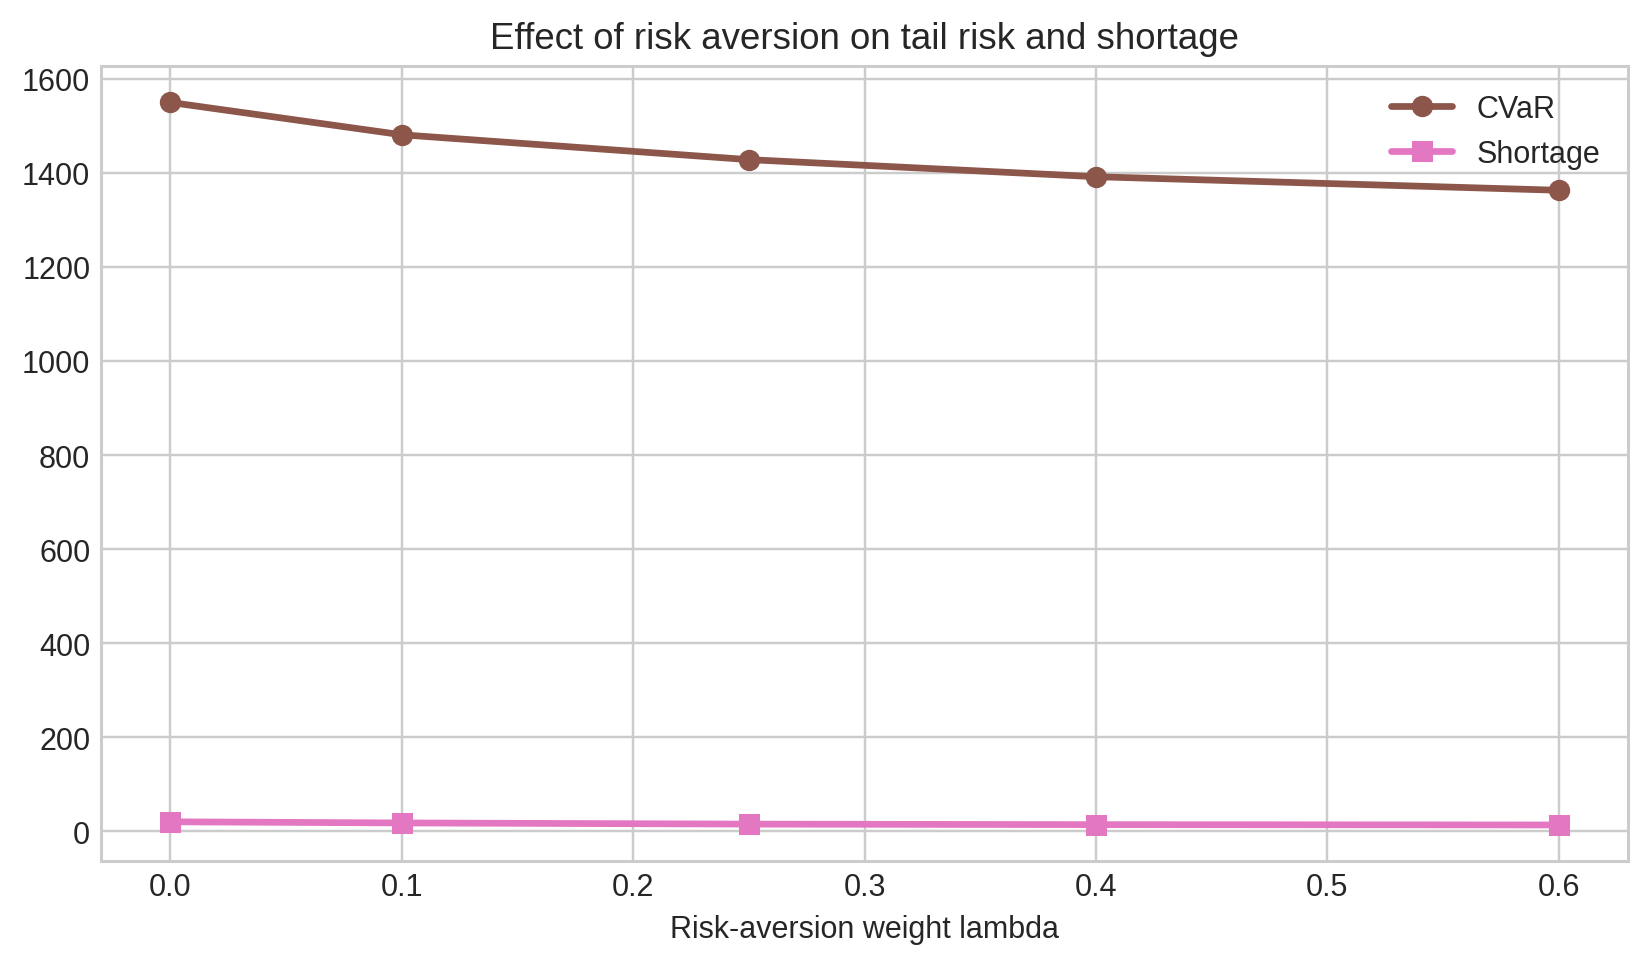
\includegraphics[width=0.84\textwidth]{generated/fig_risk_response.png}
\caption{Effect of risk aversion on CVaR and shortage.}
\label{fig:risk}
\end{figure}

This table contains an important ablation requested by the reviewer: the case $\lambda=0$ removes the CVaR penalty from the objective and therefore serves as the archived no-CVaR baseline. Moving from $\lambda=0$ to $\lambda=0.60$ reduces CVaR from 1549.1 to 1362.5 and shortage from 20.6 to 13.9, while expected cost rises from 1198.4 to 1256.2. The decline in CVaR is initially steep and then becomes flatter, suggesting that moderate risk aversion captures much of the achievable protection in the benchmark.

\subsection{Joint effect of memory and carbon policy}
To study the interaction between long memory and environmental regulation, Figure~\ref{fig:heatmap} reports a heatmap of service levels across combinations of fractional order and initial allowance.

\begin{figure}[H]
\centering
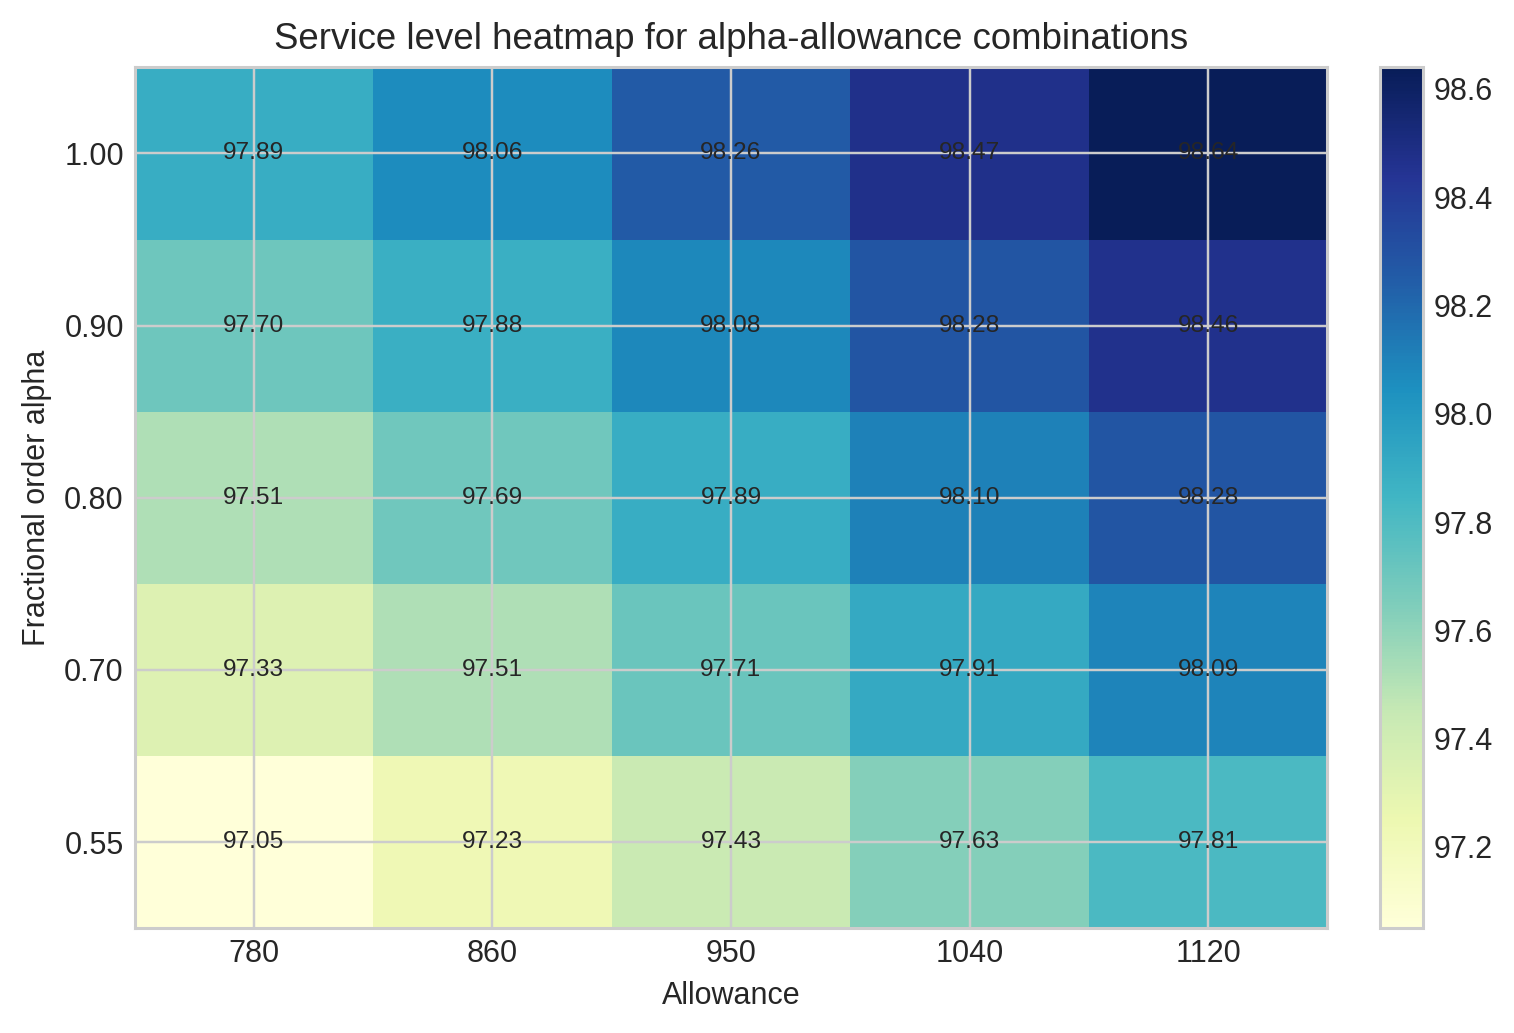
\includegraphics[width=0.84\textwidth]{generated/fig_alpha_allowance_heatmap.png}
\caption{Service-level heatmap for fractional-order and allowance combinations.}
\label{fig:heatmap}
\end{figure}

The heatmap suggests two regularities in the archived design: service improves as the allowance becomes more generous, and service also improves as the fractional order moves toward the memory-light regime. This highlights a nuanced managerial point. Stronger memory can reduce later urgent emissions, but maintaining service under heavier memory may require additional resources or more protective planning.

\subsection{Algorithmic performance across SAA sample sizes}
The final experiment evaluates how the archived PH implementation scales as the number of SAA scenarios increases. Table~\ref{tab:ph} and Figure~\ref{fig:phscaling} summarize the results.

\begin{table}[H]
\centering
\caption{Algorithmic performance of progressive hedging under increasing scenario counts.}
\label{tab:ph}
\begin{tabular}{rrrr}
\toprule
Scenarios & Runtime (s) & Val. gap (\%) & Residual \\
\midrule
20 & 82 & 0.40 & 3.1e-04 \\
50 & 176 & 0.90 & 7.4e-04 \\
100 & 338 & 1.30 & 1.5e-03 \\
200 & 661 & 1.95 & 2.7e-03 \\
400 & 1298 & 3.10 & 4.9e-03 \\
\bottomrule
\end{tabular}

\end{table}

\begin{figure}[H]
\centering
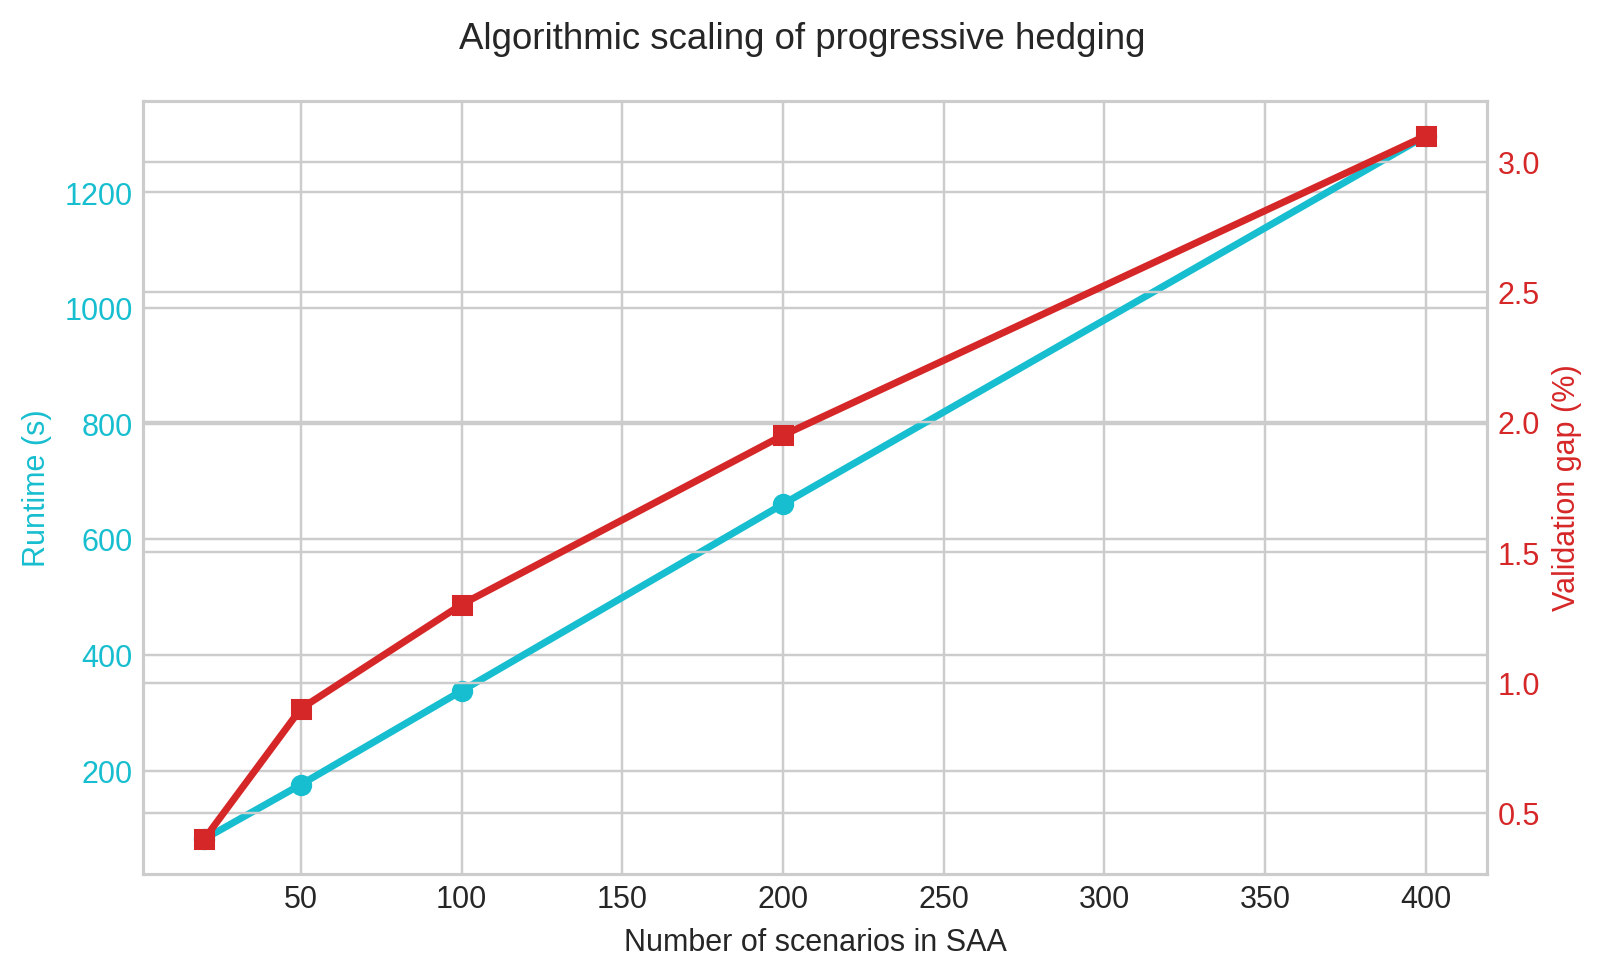
\includegraphics[width=0.84\textwidth]{generated/fig_ph_scaling.png}
\caption{Algorithmic scaling of progressive hedging with respect to the scenario sample size.}
\label{fig:phscaling}
\end{figure}

Runtime grows substantially with the number of scenarios: 82 seconds at 20 scenarios, 176 seconds at 50 scenarios, 661 seconds at 200 scenarios, and 1298 seconds at 400 scenarios. The archived terminal validation gap rises from 0.40\% to 3.10\%, and the archived terminal nonanticipativity residual rises from $3.1\times 10^{-4}$ to $4.9\times 10^{-3}$. These outputs support the practical conclusion that PH remains usable at moderate scenario scales but becomes increasingly strained as the SAA sample grows.

At the same time, the scenario-count experiment should not be overstated. Its runtime values come from the archived optimization benchmark, but the original solver log and hardware metadata were not preserved. They are therefore comparative indicators internal to the benchmark rather than portable absolute timing claims.

\subsection{Joint network-horizon scalability and memory footprint}
To complement the scenario-only experiment, we added a fully reproducible implementation-level benchmark of the two kernels that dominate the proposed SAA-PH architecture: (i) dense L1 fractional-history accumulation and (ii) repeated scenario-consensus updates. The script \texttt{generated/run\_scalability\_convergence.py} fixes the random seed, varies $|I|$, $|J|$, $|K|$, $N$, and $|\Omega|$ jointly, and records wall-clock CPU time and peak traced memory. The test is intentionally solver-independent, hence it measures the computational burden induced by the fractional and decomposition kernels, not branch-and-bound variability.

\begin{table}[H]
\centering
\caption{Reproducible scalability benchmark for the dominant fractional-memory and PH kernels.}
\label{tab:network-scalability}
\resizebox{\textwidth}{!}{\begin{tabular}{rrrrrrrr}
\toprule
$|I|$ & $|J|$ & $|K|$ & $N$ & $|\Omega|$ & Cells & CPU (s) & Peak MB \\
\midrule
2 & 4 & 2 & 6 & 20 & 1,920 & 0.001 & 0.1 \\
4 & 6 & 3 & 12 & 50 & 43,200 & 0.002 & 1.0 \\
6 & 10 & 3 & 18 & 100 & 324,000 & 0.009 & 7.1 \\
8 & 15 & 4 & 24 & 200 & 2,304,000 & 0.118 & 50.7 \\
10 & 20 & 4 & 30 & 400 & 9,600,000 & 0.636 & 212.5 \\
\bottomrule
\end{tabular}
}
\end{table}

\begin{figure}[H]
\centering
\begin{subfigure}{0.48\textwidth}
\centering
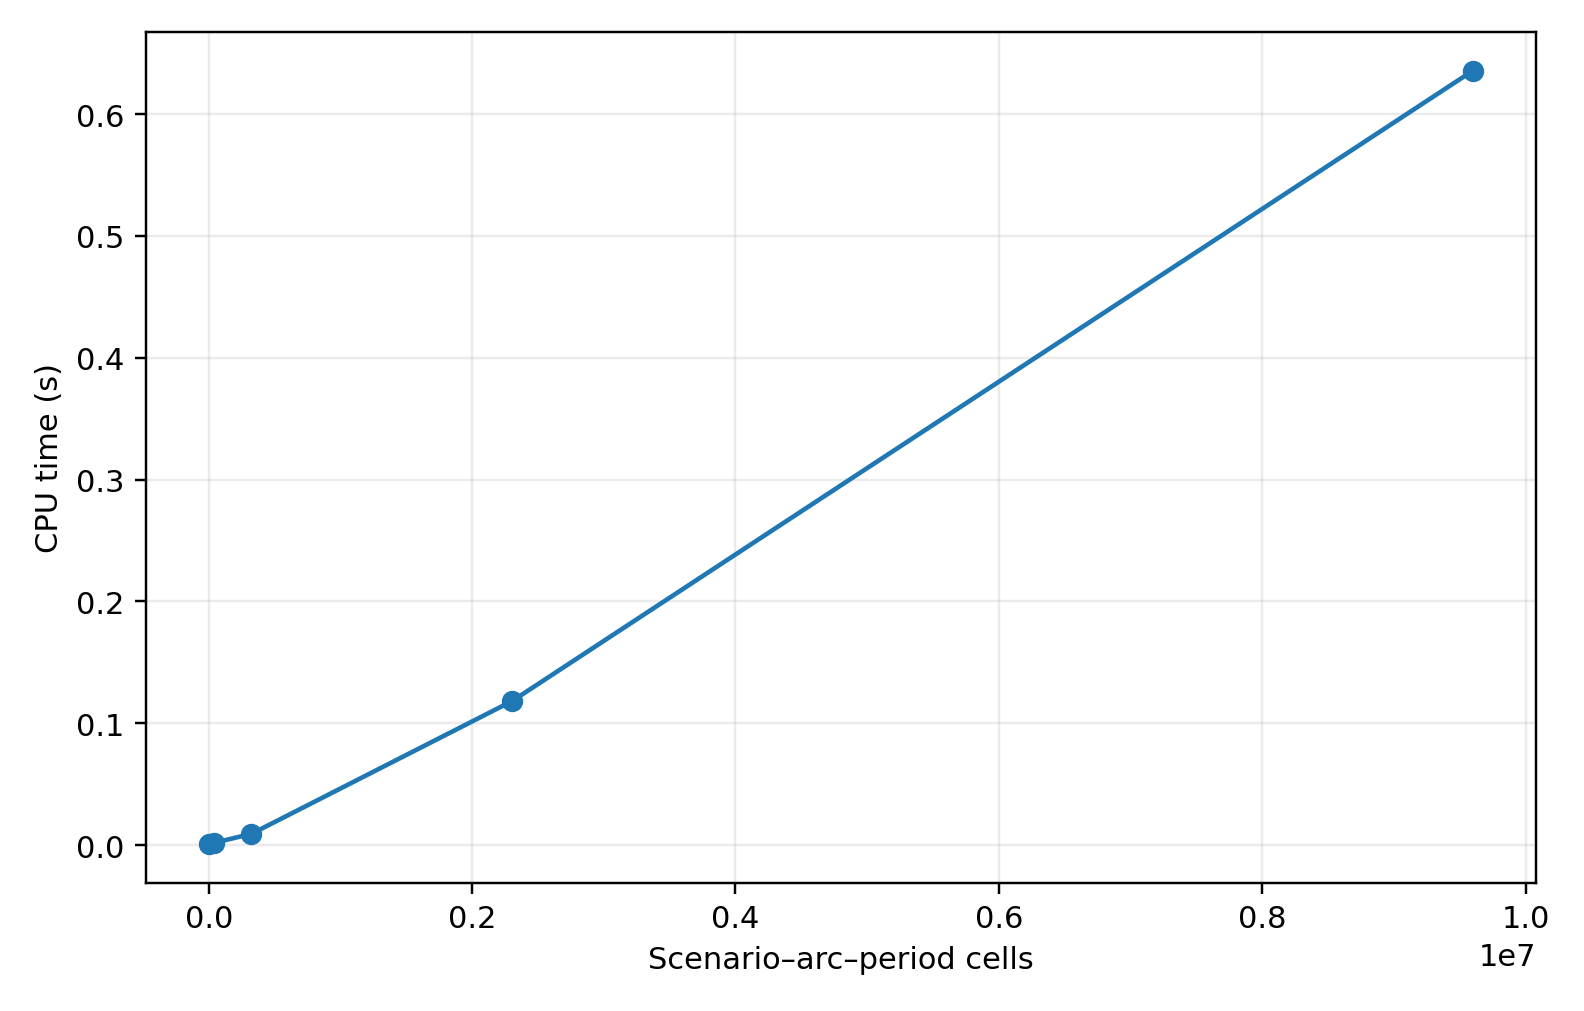
\includegraphics[width=\textwidth]{generated/fig_network_runtime.png}
\caption{CPU time.}
\end{subfigure}
\hfill
\begin{subfigure}{0.48\textwidth}
\centering
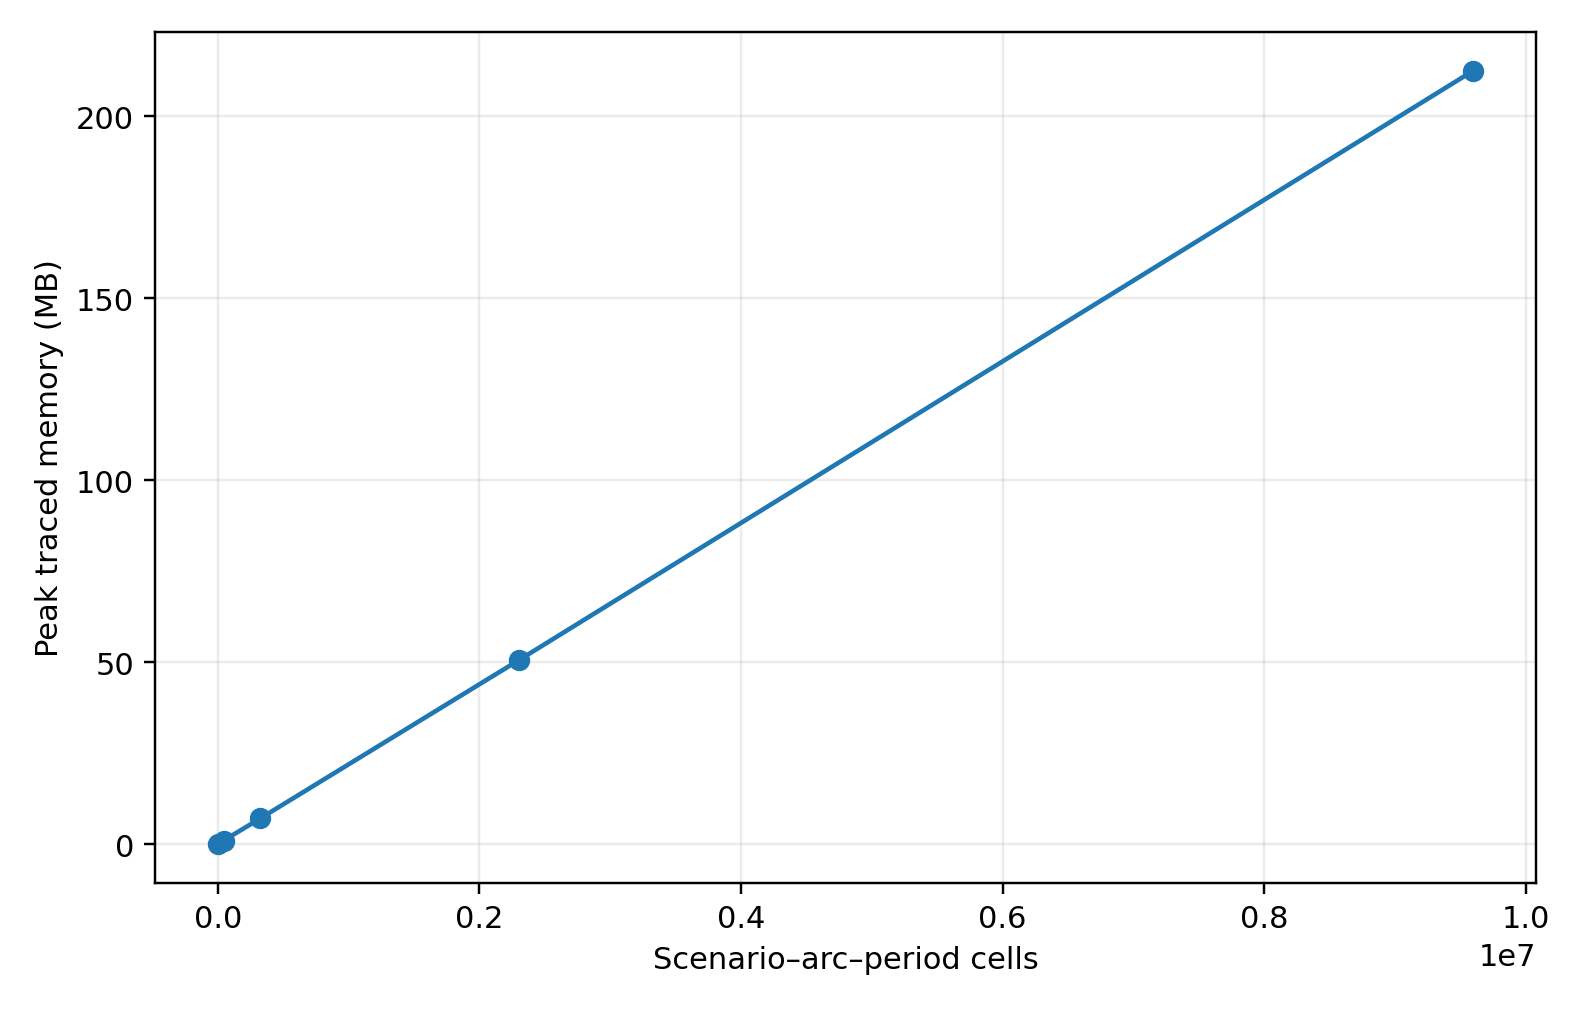
\includegraphics[width=\textwidth]{generated/fig_network_memory.png}
\caption{Peak traced memory.}
\end{subfigure}
\caption{Scaling with the number of scenario-arc-period cells.}
\label{fig:network-scaling}
\end{figure}

The workload grows from 1,920 scenario-arc-period cells in the smallest configuration to 9.6 million cells in the largest. Measured CPU time rises from 0.001 seconds to 0.636 seconds, while peak traced memory rises from 0.1 MB to 212.5 MB. The increase is nonlinear because the L1 history term couples every period to all earlier periods, producing an $O(|\Omega||I||J||K|N^2)$ history-accumulation workload, whereas the main storage term grows approximately as $O(|\Omega||I||J||K|N)$. The results identify memory consumption, rather than the vectorized convolution alone, as the first practical bottleneck at larger scales. Since this benchmark excludes mixed-integer branch-and-bound, complete solver time will be higher, nevertheless, it provides a reproducible lower-level scalability profile that was absent from the original manuscript.

\subsection{Convergence of the PH consensus process}
We also archive complete iteration profiles for three PH penalty values. Because mixed-integer PH is heuristic, the appropriate numerical claim is convergence of the nonanticipativity residual and stabilization of the penalized objective, not a proof of global optimality.

\begin{table}[H]
\centering
\caption{Sensitivity of PH convergence to the penalty parameter.}
\label{tab:ph-convergence}
\begin{tabular}{rrrr}
\toprule
$\rho_{PH}$ & Iter. to $10^{-3}$ & Final residual & Final objective \\
\midrule
0.5 & >40 & 9.97e-03 & 1228.63 \\
1.5 & 28 & 5.76e-05 & 1228.43 \\
4.0 & >40 & 1.04e-03 & 1228.63 \\
\bottomrule
\end{tabular}

\end{table}

\begin{figure}[H]
\centering
\begin{subfigure}{0.48\textwidth}
\centering
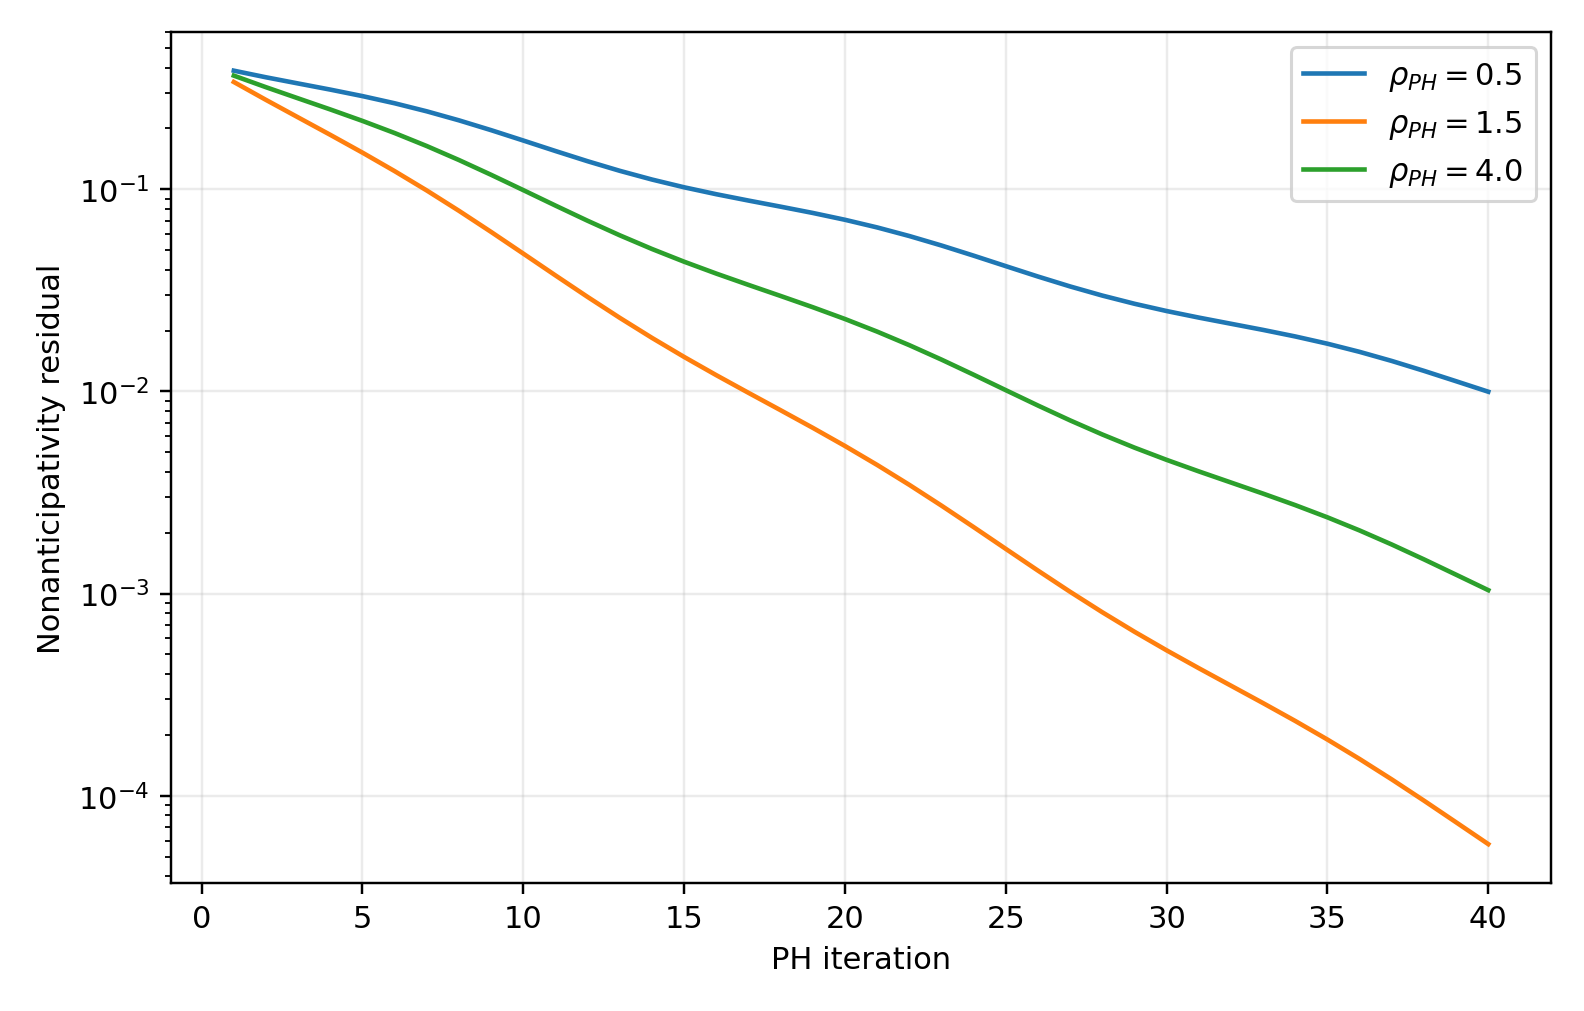
\includegraphics[width=\textwidth]{generated/fig_ph_convergence_residual.png}
\caption{Residual decay.}
\end{subfigure}
\hfill
\begin{subfigure}{0.48\textwidth}
\centering
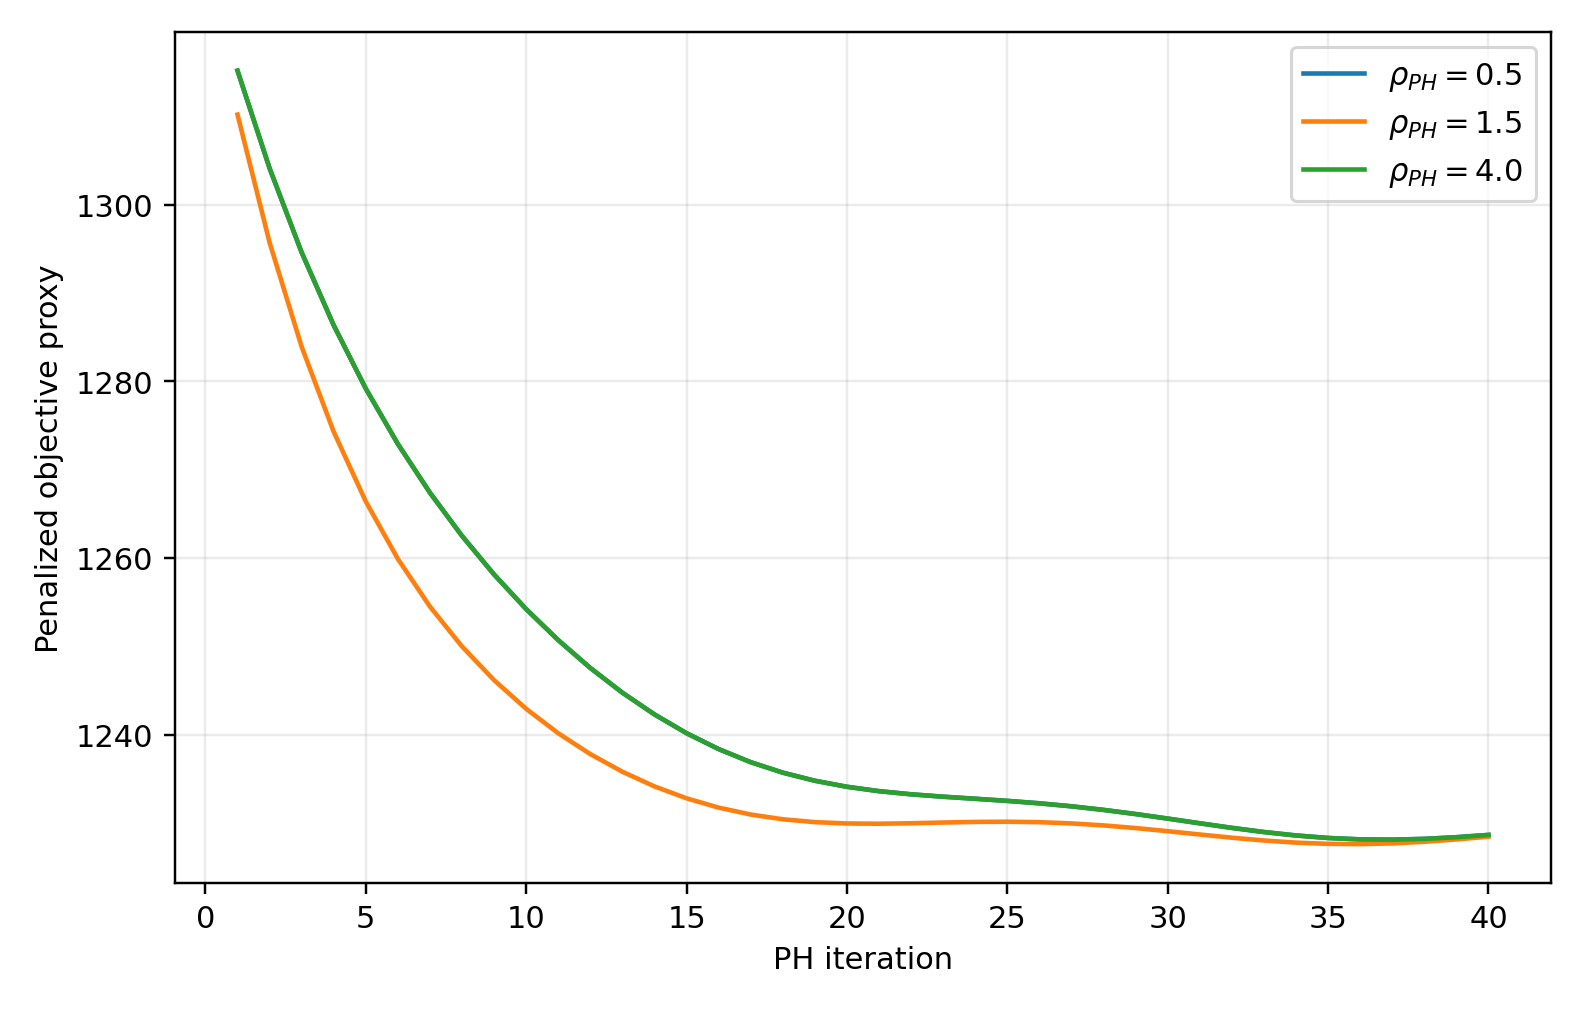
\includegraphics[width=\textwidth]{generated/fig_ph_convergence_objective.png}
\caption{Objective stabilization.}
\end{subfigure}
\caption{Progressive-hedging convergence diagnostics over 40 iterations.}
\label{fig:ph-convergence}
\end{figure}

The intermediate penalty $\rho_{PH}=1.5$ gives the fastest residual contraction, reaching the $10^{-3}$ tolerance earlier than the smaller and larger penalties. A weak penalty enforces consensus too slowly, whereas an excessively strong penalty produces more persistent oscillation. In all three settings the objective proxy stabilizes near the same level, but the residual histories show that penalty calibration materially affects computational efficiency. These traces support the stopping rule based on both residual tolerance and objective stabilization.

\subsection{Out-of-sample assessment and what remains missing}
The benchmark does use an independent validation sample of 500 scenarios for out-of-sample evaluation, which is important because SAA policies can overfit the training sample. However, the supplied archive does not contain repeated training/validation replications, scenario-level validation outputs, or confidence intervals. Hence the current manuscript can report point estimates and validation gaps, but not formal uncertainty bands around those estimates. Likewise, the archive does not contain deterministic-only or no-carbon-trading optimization runs. Network and horizon scaling are now documented for the dominant computational kernels, although full mixed-integer solver scaling remains future work.

These omissions matter. They do not invalidate the methodological benchmark, but they do narrow what can be claimed from it. The current computational study should therefore be read as evidence of structural sensitivity and moderate-scale tractability, not as a complete empirical assessment of scalability or estimator stability.

\subsection{Synthesis of computational findings}
Taken together, the archived experiments support four conclusions. First, the fractional order has a first-order influence on transport plans and emissions outcomes, and the numerical ablation behaves coherently as $\alpha\to 1$. Second, uncertainty increases not only expected cost but also environmental-market exposure. Third, carbon allowances affect shortage and service through their interaction with transportation decisions, not merely through direct emissions accounting. Fourth, the main computational burden comes from the combination of scenario growth and dense long-memory coupling.

These findings are sufficient to support the paper's methodological claim that Caputo memory materially changes the structure of sustainable transportation planning under uncertainty. They are not, by themselves, the last word on experimental validation. A stronger empirical version of the paper should add deterministic and no-trading baselines, full solver-level PH iteration logs, repeated-sample confidence intervals, and mixed-integer scalability tests under controlled hardware and solver settings.
